\newpage
\section{Linear Equations with Infinite Domains}

\subsection{Transport Equation}

\begin{enumerate}
  \item The Transport Equation
  %
  \begin{align}
    u_t & = cu_x
  \end{align}
  \begin{enumerate}
    \item First order equation
    \item $x \in (-\infty, \infty)$
    \item $t \in [0, \infty)$
    \item In essence, $u(x, 0) = f(x)$
  \end{enumerate}
\end{enumerate}
  \bigbreak

  Here, let us guess $u(x, t) = v(x + ct)$. Solutions of this form are called travelling wave equations.

  Here, let us establish $\eta = x + ct$

  When finding our partials, we run through the following tree:

  \begin{center}
    $u$\\
    $|$\\
    $v$\\
    $\eta$\\
    $| \quad |$\\
    $x \quad t$
  \end{center}

  Let's show that this satisfies $u_t = cu_x$.
  %
  \begin{align}
    \frac{\p u}{\p t} & = \frac{\p v}{\p t} = \frac{dv}{d\eta} \frac{\p \eta}{\p t} = \frac{dv}{d \eta} \cdot c\\
    \frac{\p u}{\p x} & = \frac{\p v}{\p t} = \frac{dv}{d \eta} \frac{\p \eta}{\p x} = \frac{dv}{d \eta} \cdot 1\\
    u_t & = cu_x
  \end{align}

  Any function of the form $u = v(x + ct)$ is a solution to $u_t = cu_x$.

  Let's look at the initial condition:
  %
  \begin{align}
    u(x, 0) & = f(x)\\
    u(x, 0) & = v(x)
  \end{align}
  Here, $v(x) = f(X)$. In addition, $u = v(x + ct) = f(x + ct)$.

  \ex%
  \begin{align}
    u_t & = -3u_X\\
    u(x, 0) & = e^{-x^2}\\
    u(x, t) & = e^{-(x - 3t)^2}
  \end{align}

\begin{center}
  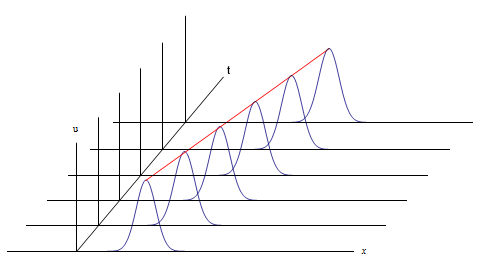
\includegraphics{Transport Equation.png}
\end{center}

The solution translates as time increases, which is why it's called a travelling wave solution.

In this particular case, if $x - 3t = $ constant, then $u$ is fixed.

\underline{Remarks}
%
\begin{enumerate}
  \item The parallel lines are called characteristic curves
  \item The slope of the characteristic line is $-\frac{1}{c}$ for $u_t = cu_x$.
  $c$ is the speed of the solution.
  It tells us how fast the waves are translated in the $x-$direction.
\end{enumerate}

\underline{Lemma}
%
\begin{align}
  \int^\infty_{-\infty} e^{-x^2} \text{ dx} & = \sqrt \pi
\end{align}

\begin{proof}
  Let us look at our equation squared:
  %
  \begin{align}
    I^2 & =
    \int^\infty_{-\infty} e^{-x^2} \text{ dx} \cdot
    \int^\infty_{-\infty} e^{-y^2} \text{ dy}\\
    & = \int^\infty_{-\infty} \int^\infty_{-\infty}
    e^{-x^2} \cdot e^{-y^2} \text{ dx dy}\\
    & =
    \int^\infty_{-\infty} \int^\infty_{-\infty}
    e^{-x^2 - y^2} \text{ dx dy}\\
    & =
    \int^{2 \pi}_{0} \int^\infty_0
    e^{-r^2} r \text{ dr d}\theta
  \end{align}

  Here, use polar to find our integral.
\end{proof}

\topic{March 2, 2022}
%
\begin{align}
  I & = \int^\infty_{-\infty} e^{-x^2} \text{ dx} = \sqrt{\pi}
\end{align}

Let $u = r^2$
%
\begin{align}
  I^2 & = \int^{2\pi}_0 \int^\infty_0 e^{-r^2} r \text{ dr d}\theta\\
  & = \int^{2\pi}_0 -\frac{1}{2} e^{-r^2} \Big|^\infty_0 \text{ d}\theta\\
  & = \int^{2 \pi}{0} \frac{1}{2} \text{ d}\theta\\
  & = \frac{1}{2} \cdot 2 \pi\\
  & = \pi
\end{align}

Solving Linear Constant Coefficient PDEs with Fourier Transform

Assume $u(x, t)$ with $x \in (-\infty, \infty)$
\begin{enumerate}
  \item Fourier Transform with respect to $x$
  \item Solve the resulting ODE in $T$
  \item Retransform to go back into real space.
\end{enumerate}

We need $\displaystyle \lim_{x \to \pm \infty} u(x, t) = 0$. This will replace the boundary conditions we have used before.

\bigbreak

\subsection{Laplace Equation}
\begin{itemize}
  \item $u_{xx} + u_{yy} = 0$
  \item $x \in (-\infty, \infty)$
  \item $y \in (-\infty, \infty)$
  \item $\displaystyle \lim{x \to \pm \infty}{y \to \pm \infty} u(x, y) = 0$
  %\dlim was spotted here ^
\end{itemize}
Here, the solution is $u(x, y) = 0$. Using MVT (use ball with large radius).

\bigbreak

\subsection{Heat Equation}

Let us consider the following conditions:
%
\begin{itemize}
  \item $u_t = u_{xx}$
  \item $u(x, 0) = f(x)$
  \item $\displaystyle \lim_{x \to \pm \infty} u(x, t) = 0$
  \item $t \in [0, \infty)$
  \item $x \in (-\infty, \infty)$
\end{itemize}

Now, let us consider the following steps:
%
\begin{enumerate}
  \item Solve for $u_t = u_{xx}$
  %
  \begin{align}
    u_t & = u_{xx}\\
    F[u_t] & = F[u_{xx}]\\
    \frac{1}{\sqrt{2 \pi}} \int^\infty_{-\infty} u_t e^{-i x \xi} \text{ dx} & = \frac{1}{\sqrt{2 \pi}} \int^\infty_{-\infty} u_{xx} e^{-i x \xi} \text{ dx}\\
    %
    \frac{\p}{\p t} \left[ \frac{1}{\sqrt{2 \pi}} \int^\infty_{-\infty} u e^{-i x \xi} \text{ dx} \right]
    & = (i \xi)^2 \frac{1}{\sqrt{2 \pi}} \int^\infty_{-\infty} u e^{-i x \xi} \text{ dx}\\
    %
    \frac{\p}{\p t} \hat u(\xi, t) & = - \xi^2 \hat u(\xi, t)
  \end{align}

  Our initial condition becomes:
  %
  \begin{align}
    F[u(x, 0)] & = \frac{1}{\sqrt{2 \pi}} \int^\infty_{-\infty} u(x, 0) e^{-i x \xi} \text{ dx}\\
    & = \frac{1}{\sqrt{2 \pi}} \int^\infty_{-\infty} f(x) e^{-i x \xi} \text{ dx}\\
    & = \hat f(\xi)
  \end{align}
  %
  \item Solve $\hat u_t = -\xi^2 \hat u$, $\hat u(\xi, 0) = \hat f(\xi)$. Here, let us write the general form of $\hat u$:
  %
  \begin{align}
    \hat u(\xi, t) & = A(\xi) e^{- \xi^2 t}
  \end{align}

  Here, let us use our initial condition to find $A(\xi)$
  %
  \begin{align}
    \hat u (\xi, 0) \hat f(\xi) & = A(\xi)\\
    \hat u(\xi, t) & = \hat f(\xi) e^{-\xi^2 t}
  \end{align}

  \item Retransform
  %
  \begin{align}
    u(x, t) & = \frac{1}{\sqrt{2 \pi}} \int^\infty_{-\infty} \hat u(\xi, t) e^{-i x \xi} \text{ d}\xi\\
    & = \frac{1}{\sqrt{2 \pi}} \int^\infty_{-\infty} \hat f(\xi) e^{-\xi^2 t}e^{i x \xi} \text{ d}\xi\\
    & = \frac{1}{\sqrt{2 \pi}} \int^\infty_{-\infty}
    \color{blue}{\frac{1}{\sqrt{2 \pi}} \int^\infty_{-\infty} f(y) e^{-i y \xi} \text{ dy}} \ \color{black}
    e^{-\xi^2 t} e^{i x \xi} \text{ d}\xi\\
    & = \frac{1}{2 \pi} \int^\infty_{-\infty} \int^\infty_{-\infty}
    f(y)e^{-i y \xi} e^{-\xi^2 t} e^{i x \xi} \text{ dy d}\xi\\
    & = \frac{1}{2 \pi} \int^\infty_{-\infty} f(y)
    \int^\infty_{-\infty} e^{-i y \xi} e^{-\xi^2 t} e^{i x \xi} \text{ d}\xi \text{ dy}\\
    & = \frac{1}{2 \pi}
    \int^\infty_{-\infty} f(y)
    \color{red}
    \int^\infty_{-\infty} e^{-\xi^2 t + i \xi(x - y)} \text{ d}\xi
    \color{black}
    \text{ dy}
  \end{align}

  Here, let us focus our attention on the inner integral, where we rewrite it as \textcolor{red}{Q}.
  %
  \begin{align}
    Q & = \int^\infty_{-\infty} e^{-\xi^2 t + i\xi(x - y)} \text{ d}\xi
  \end{align}

  Let's look at the following:
  %
  \begin{align}
    -\xi^2 t + i\xi(x - y) & = -t\left[ \xi^2 - \frac{i \xi(x - y)}{t}\right]\\
    & = -t \left[ \left(\xi - \frac{i(x - y)}{2t}\right)^2 - \frac{i^2(x - y)^2}{4t^2} \right]\\
    & = -t \left[ \left(\xi - \frac{i(x - y)}{2t}\right)^2 + \frac{(x - y)^2}{4t^2} \right]
  \end{align}

  Now, we have the following for Q:
  %
  \begin{align}
    Q & = \int^\infty_{-\infty} e^{-t \left[ \left(\xi - \frac{i(x - y)}{2t}\right)^2 + \frac{(x - y)^2}{4t^2} \right]} \text{ d}\xi\\
    & = \int^\infty_{-\infty} e^{-t\left( \xi - \frac{i(x - y)}{2t}\right)^2 - \frac{(x - y)^2}{4t}} \text{ d}\xi\\
    & = \int^\infty_{-\infty} e^{-t \left(\xi - \frac{i(x - y)}{2t}\right)^2} e^{- \frac{(x - y)^2}{4t}} \text{ d}\xi\\
    & = e^{- \frac{(x - y)^2}{4t}} \int^\infty_{-\infty} e^{-t \left(\xi - \frac{i(x - y)}{2t}\right)^2} \text{ d}\xi
  \end{align}

  Here, let us consider the following substitution:
  %
  \color{blue}
  \begin{align}
    w & = \sqrt t \left( \xi - \frac{i(x - y)}{2t}\right)\\
    dw & = \sqrt t \text{ d}\xi
  \end{align}
  \color{black}

  Now, let us write:
  %
  \begin{align}
    e^{- \frac{(x - y)^2}{4t}} \frac{1}{\sqrt t} \int^{\textcolor{blue}{\infty}}_{\textcolor{blue}{-\infty}} e^{-w^2} \text{ dw}
    & = \sqrt{\frac{\pi}{t}} e^{- \frac{(x - y)^2}{4t}}\\
    u(x, t) & = \frac{1}{2 \pi} \int^\infty_{- \infty} f(y) \sqrt{\frac{\pi}{t}} e^{- \frac{(x - y)^2}{4t}} \text{ dy}\\
    & = \frac{1}{2 \sqrt{\pi t}} \int^\infty_{-\infty} f(y) e^{- \frac{(x - y)^2}{ty}} \text{ dy}
  \end{align}
\end{enumerate}

\subsection{Wave Equation}

\topic{March 4, 2022}

Here, let us consider the following conditions:
%
\begin{itemize}
  \item $u_{tt} = u_{xx}$, $t \in [0, \infty), x \in (-\infty, \infty)$
  \item $\displaystyle \lim_{x \to \pm \infty} u(x, t) = 0$
  \item $u(x, 0) = f(x)$
  \item $u_t(x, 0) = g(x)$
\end{itemize}

\note Two initial conditions for wave: Heat's condition $(u(x, 0) = f(x))$ and $u_t(x, 0) = g(x)$

Now, let us begin:
%
\begin{enumerate}
  \item Let us solve $F$:
  %
  \begin{align}
    F[u_{tt}] & = F[u_{xx}]\\
    \Rightarrow \hat u_{tt} & = (i \xi)^2 \hat u\\
    \Rightarrow \hat u_{tt} & = - \xi^2 \hat u\\
    \hat u(\xi, 0) & = \hat f(\xi)
  \end{align}

  Now, let us consider $\hat u_t(\xi, 0)$:
  %
  \begin{align}
    F[u_t(x, 0)] & = \frac{1}{\sqrt{2 \pi}} \int^\infty_{-\infty} u_t(x, 0) e^{-i x \xi} \text{ dx}\\
    & = \frac{1}{\sqrt{2 \pi}} \int^\infty_{-\infty} g(x) e^{-i x \xi} \text{ dx}\\
    & = \hat g(\xi)
  \end{align}

  \item Solve $\hat u_{tt} = -\xi^2 \hat u$ with the following conditions:
  \begin{itemize}
    \item $\hat u(\xi, 0) = \hat f(\xi)$
    \item $\hat u_t(\xi, 0) = \hat g(\xi)$
  \end{itemize}

  Now let us write the general form:
  %
  \begin{align}
    \hat u(\xi, t) & = A(\xi) \sin(\xi t) + B(\xi) \cos(\xi t)
  \end{align}

  Here, we do not want to use sine and cosine because we will multiply by expontentials later on.
  %
  \begin{align}
    \hat u(\xi, t) & = A(\xi) e^{i \xi t} + B(\xi) e^{-i \xi t}\\
    \hat u(\xi, 0) & = A(\xi) + B(\xi) = \hat f(\xi)
  \end{align}

  Here, let us find the $t$ partial,
  %
  \begin{align}
    \hat u_t(\xi, t) & = i \xi A(\xi) e^{i \xi t} - i \xi B(\xi) e^{- i \xi t}\\
    \hat u (\xi, 0) & = i \xi A(\xi) - i \xi B(\xi) = \hat g(\xi)
  \end{align}

  Here, let us take the equation with $\hat f(\xi)$ and multiply it by $i \xi$:
  %
  \begin{align}
    2 i \xi A(\xi) & = i \xi \hat f(\xi) + \hat g (\xi)\\
    a(\xi) & = \frac{\hat f(\xi)}{2} + \frac{\hat g(\xi)}{2 i \xi}
  \end{align}

  Now, let us subtract to find $B$:
  %
  \begin{align}
    2 i \xi B(\xi) & = i \xi \hat f (\xi) - \hat g (\xi)\\
    B(\xi) & = \frac{\hat f(\xi)}{2} - \frac{\hat g(\xi)}{2 i \xi}
  \end{align}

  Here, substitute in our terms:
  %
  \begin{align}
    \hat u(\xi, t)
    & = \left[ \frac{\hat f(\xi)}{2} + \frac{\hat g(\xi)}{2 i \xi}  \right] e^{i \xi t} + \left[ \frac{\hat f(\xi)}{2} - \frac{\hat g(\xi)}{2 i \xi} \right] e^{-i \xi t}
  \end{align}

  \item Retransform
  %
  \begin{align}
    u(x, t)
    & = \frac{1}{\sqrt{2 \pi}} \int^\infty_{-\infty} \hat u(\xi, t) e^{i x \xi} \text{ d}\xi\\
    & = \frac{1}{\sqrt{2 \pi}} \int^\infty_{-\infty} \left[ \frac{\hat f(\xi)}{2} + \frac{\hat g(\xi)}{2 i \xi}  \right] e^{i \xi t} + \left[ \frac{\hat f(\xi)}{2} - \frac{\hat g(\xi)}{2 i \xi} \right] e^{-i \xi t} \text{ d}\xi\\
    & =
    \frac{1}{2 \sqrt{2 \pi}} \int^\infty_{-\infty}
    \hat f(\xi)
    \left(e^{i \xi t} + e^{-i \xi t}\right)e^{i x \xi} +
    \frac{\hat g(\xi)}{i \xi}
    \left( e^{i \xi t} - e^{-i \xi t} \right)e^{i x \xi} \text{ d}\xi\\
    & =
    \frac{1}{2 \sqrt{2 \pi}} \int^\infty_{-\infty}
    \hat f(\xi) \left[ e^{i \xi(x + t)} + e^{i \xi(x - t)} \right] \text{ d}\xi
    + \frac{1}{2 \sqrt{2 \pi}} \int^\infty_{-\infty}
    \frac{\hat g(\xi)}{i \xi}
    \left[ e^{i \xi(x + t)} - e^{i \xi(x - t)} \right] \text{ d}\xi
  \end{align}

  We know that
  %
  \begin{align}
    f(x) & = \frac{1}{\sqrt{2 \pi}} \int^\infty_{-\infty} \hat f(\xi) e^{i x \xi} \text{ d}\xi\\
    f(x + t) & = \frac{1}{\sqrt{2 \pi}} \int^\infty_{-\infty} \hat f(\xi) e^{i \xi(x + t)} \text{ d}\xi\\
    f(x - t) & = \frac{1}{\sqrt{2 \pi}} \int^\infty_{-\infty} \hat f(\xi) e^{i \xi(x - t)} \text{ d}\xi
  \end{align}

  From the previous two equations, let us write:
  %
  \begin{align}
    \frac{1}{2} \left[ f(x + t) + f(x - t) \right]
    & = %\frac{1}{2} \left[ f(x + t) + f(x - t) \right] +
    \frac{1}{2 \sqrt{2 \pi}} \int^\infty_{-\infty} \frac{\hat g(\xi)}{i \xi} \left( e^{i \xi(x + t)} - e^{i \xi(x - t)} \right) \text{ d}\xi
  \end{align}

  Now, let us write:
  %
  \begin{align}
    \frac{\hat g(\xi)}{i \xi}
    & = \frac{\frac{1}{\sqrt{2\pi}} \int^\infty_{-\infty} g(x)e^{-i x \xi} \text{ dx}}{i \xi}\\
    & = \frac{1}{\sqrt{2 \pi}} \int^\infty_{-\infty} \frac{g(x)e^{-i x \xi} }{i \xi} \text{ dx}
  \end{align}

  Here, we consider integral by parts: $u = \frac{e^{- x \xi}}{- i \xi} \Rightarrow du = e^{- i \xi} \text{ dx}$ and $dv = g(x) \text{ dx} \Rightarrow v = \int^x_{-\infty} g(y) \text{ dy}$.
  %
  \begin{align}
    & = - \frac{1}{\sqrt{2 \pi}}
    \left[
    \int^x_{-\infty} g(y) \text{ dy } \frac{e^{-i \xi x}}{- i \xi} \Big|^\infty_{-\infty} - \int^\infty_{-\infty} \int^x_{-\infty} g(y) \text{ dy } e^{-i x \xi} \text{ dx}
    \right]\\
    & = \hat h(\xi)
  \end{align}

  Now, from the two equations, let us consider $f(x - t)$:
  %
  \begin{align}
    & = \frac{1}{2} \left[ f(x + t) + f(x - t) \right] + \frac{1}{2 \sqrt{2 \pi}} \int^\infty_{-\infty} \hat h(\xi) \left( e^{i \xi(x + t)} - e^{i \xi(x - t)} \right)\ text{ d}\xi\\
    & = \frac{1}{2} \left[ f(x + t) + f(x - t) \right] + \frac{1}{2} \left[ h(x + t) - h(x - t)\right]\\
    & = \frac{1}{2} \left[ f(x + t) + f(x - t) \right]
    + \frac{1}{2} \left[ \int^{x + t}_{- \infty} g(y) \text{ dy } - \int^{x - t}_{-\infty} g(y) \text{ dy} \right]\\
    & = \frac{1}{2} \left[ f(x + t) + f(x - t) \right]
    + \frac{1}{2} \int^{x + t}_{x - t} g(y) \text{ dy}
  \end{align}

  This is the solution to the wave equation on an infinite domain called D'Alembert's Formula.
  %
\end{enumerate}

\subsection{Wave Equation Solutions}

\topic{March 7, 2022}
%
\begin{itemize}
  \item $u_{tt} = c^2 u_{xx}$
  \item $x \in (-\infty, \infty), t \in [0, \infty)$
  \item $u(x, 0) = f(x)$
  \item $u_t(x, 0) = g(x)$
  \item $\displaystyle u(x, t) = \frac{1}{2} \left[ f(x + ct) + f(x - ct) \right] + \frac{1}{2c} \int^{x + ct}_{x - ct} g(y) \text{ dy}$
\end{itemize}
%
\begin{enumerate}
  \item Conservation of Energy
  %
  \begin{align}
    \frac{dE}{dt} & = 0
  \end{align}

  Here, let us consider the energy as:
  %
  \begin{align}
    E & = \frac{1}{2} \int^\infty_{-\infty} (u^2_t + c^2 u^2_x) \text{ dx}
  \end{align}

  Here, the first term is kinetic energy and the second term is the potential energy. Let us derive our $E$:
  %
  \begin{align}
    \frac{dE}{dt}
    & = \frac{d}{dt} \frac{1}{2} \int^\infty_{-\infty} (u^2_t + c^2 u^2_x) \text{ dx}\\
    & = \frac{1}{2} \int^\infty_{-\infty} 2u_t u_{tt} + 2 c^2 u_x u_{xt} \text{ dx}\\
    & = \int^\infty_{-\infty} u_t u_{tt} + c^2 u_x u_{xt} \text{ dx}\\
    & = \int^\infty_{-\infty} u_t c^2 u_{xx} + c^2 u_x u_{xt} \text{ dx}\\
    & = c^2 \int^\infty_{-\infty} u_t u_{xx} + u_x u_{xt} \text{ dx}
  \end{align}

  Here, let us integrate $u_{xx}$ and differentiate $u_t$:
  %
  \begin{align}
    c^2
    \left[
     u_t u_x \Big|^\infty_{-\infty} + \int^\infty_{-\infty} - u_{tx} u_x + u_x u_{xt} \text{ dx}
    \right]
    & = 0
  \end{align}

  Here, this shows our conservation of energy.
  %
  \item \topic{Domain of Dependence / Range of Influence}

  How does the solution at a point depend on the initial condition?
  % Image

  The domain of dependence is the interval between these two points:
  %
  \begin{align}
    [x_0 - ct_0, x_0 + ct_0]
  \end{align}

  If we change the initial condition of a point, where will $u$ be altered?

  The range of influence of the initial condition at point $x_0$ is
  %
  \begin{align}
    \left\{ (x, t) : \frac{| x - x_0|}{t} \leq c \right\}
  \end{align}
  %
  \item Parallelogram Property (Also valid on $x \in [a, b]$).
  %
  % Image
  %     D -1/c Slope
  %       C
  %  B    1/c Slope
  %   A
  %
  \begin{center}
    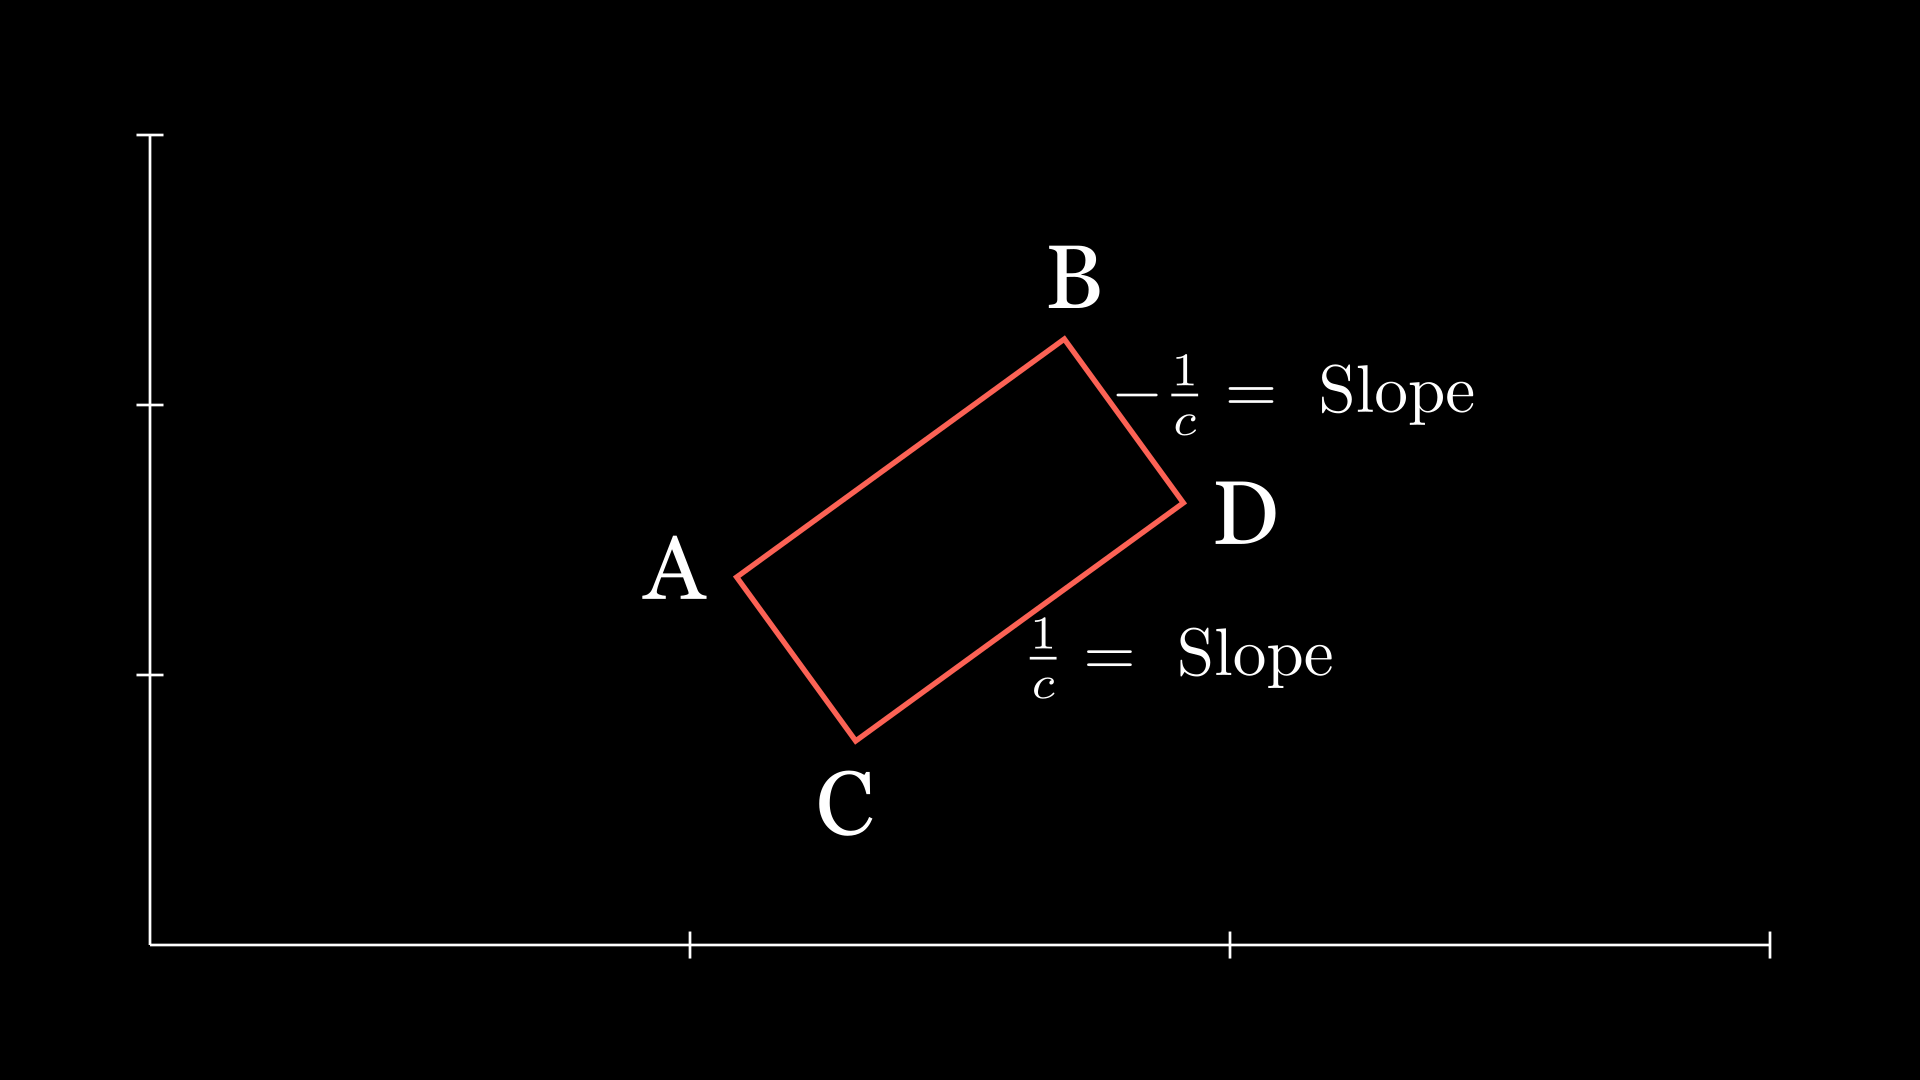
\includegraphics[height = 4cm]{Heat Equation Solution Rectangle}
  \end{center}
  \begin{align}
    u(A) + u(D) & = u(B) + u(C)
  \end{align}

  \item Reversal of Time

  You can solve the wave equation in backward time
  %
  \begin{enumerate}
    \item $x \in (-\infty, \infty)$
    \item $x \in [a, b]$
    \item $x \in \Omega \subseteq \R^n$
  \end{enumerate}

  \item Expanding to Multi-Dimensions

  We cannot expand D'Alembert's Formula in any way to $x \in \R^n, n \leq 2$.

  There are formulas for solving the wave equation for $n \leq 2$.

  The wave equation and the transport equation are both called hyperbolic equations because characteristics are involved in the solution of both.

  Here, let us write:
  %
  \begin{center}
    \begin{tabular}{l|l}
      Transport & $x + ct$\\
      Wave & $x + ct, x - ct$
    \end{tabular}\\
    \smallbreak
    \begin{tabular}{l|ll}
      Transport & $u_t = cu_x$ & $u(x, 0) = f(x)$\\
      Wave & $U_t = CU_x$ & $U(x, 0) = F(x)$
    \end{tabular}\\
    Where $U =
    \begin{bmatrix}
      u_t\\
      u_x
    \end{bmatrix}
    $
  \end{center}

  Now, let us consider:
  %
  \begin{align}
    U_t = CU_x \Rightarrow
    \begin{bmatrix}
      u_{tt}\\
      u_{xt}
    \end{bmatrix}
    & =
    \begin{bmatrix}
      0 & c^2\\
      1 & 0
    \end{bmatrix}
    \begin{bmatrix}
      u_{tx}\\
      u_{xx}
    \end{bmatrix},\\
    U(x, 0) & =
    \begin{bmatrix}
      u_t(x, 0)\\
      u_x(x, 0)
    \end{bmatrix}
    =
    \begin{bmatrix}
      g(x)\\
      f^\prime(x)
    \end{bmatrix}
  \end{align}
\end{enumerate}

%\topic{Wave Equation Solutions}

\topic{March 9, 2022}

%
\begin{itemize}
  \item $u_t = u_xx$
  \item $x \in (-\infty, \infty)$, $t \in [0, \infty)$
  \item $u(x, 0) = f(x)$
  \item $\displaystyle u(x, t) = \frac{1}{\sqrt{4 \pi t}} \int^\infty_{-\infty} f(y) e^{- \frac{(x - y)^2}{4t}} \text{ dy}$
\end{itemize}

Let the initial condition be a ``delta function,'' $\delta(x)$.

\bigbreak

\emph{What is a delta function, $\delta(x)$?}

It has two main properties:
%
\begin{enumerate}
  \item $\delta(x) = 0$, $x \neq 0$.
  \item $\displaystyle \int^\infty_{-\infty} \delta(x) \text{ dx } = 1$
\end{enumerate}

The ``mass'' is centered at $x = 0$. The delta function is not a function because $\delta(0) = ?$. Actually, the delta function is a measure.

\subsubsection{Calculations with Delta Functions}
%
\begin{align}
  \int^\infty_{-\infty} \delta(y) g(x - y) \text{ dy}
  & = \int^\infty_{-\infty} \delta(x- y) g(y) \text{ dy} = g(x)
\end{align}

Here, $\delta(y)$ is zero except when $y = 0$ and $\delta(x - y) = 0$ except when $x = y$.

Here, we have a convolution $\delta * g$, where our variables can switch.

What do we expect when $f(x) = \delta(x)$?

When $t = 0$, our area is the $t$ axis: $|$, however, as $t \to \infty$, then the area slowly flattens, akin to a candle.

Mathematically, what do we expect?
%
\begin{align}
  u(x, t) & = \frac{1}{\sqrt{4 \pi t}} \int^\infty_{-\infty} \delta(y) e^{- \frac{(x - y)^2}{4t}} \text{ dy}\\
  & = \frac{1}{\sqrt{4 \pi t}} e^{- \frac{x^2}{4 t}}
\end{align}

The $t$'s impact in the fraction reduces the amplitude and the $t$ in the exponent flattens out the curve.

This is the Gaussian Normal Distributions

What if $f(x) = 7 \delta(x) + 5 \delta(x - 3)$?
%
\begin{align}
  u(x, t) & = \frac{1}{\sqrt{4 \pi t}} \int^\infty_{-\infty} [7 \delta(y) + 5 \delta(y - 3)] e^{-\frac{(x - y)^2}{4 t}} \text{ dy}\\
  & = \frac{1}{\sqrt{4 \pi t}}
  \left[
    \int^\infty_{-\infty} 7 \delta(y) e^{- \frac{(x - y)^2}{4 t}} \text{ dy} +
    \int^\infty_{-\infty} 5 \delta(y - 3) e^{-\frac{(x - y)^2}{4t}} \text{ dy}
  \right]\\
  & = \frac{1}{\sqrt{4 \pi t}}
  \left[
    7e^{- \frac{x^2}{4 t}} + 5 e^{-\frac{(x - 3)^2}{4 t}}
  \right]
\end{align}

So for a general $f(x)$, think of $f(x)$ as a bunch of delta functions.

%______________________________________________________________________________%

\topic{Conservation of Energy}

The amount of heat stamp? constant
%
\begin{align}
  \frac{d}{dt} \int^\infty_{-\infty} u(x, t) \text{ dx}
  & = \int^\infty_{-\infty} u(x, t) \text{ dx}\\
  & = \alpha^2 \int^\infty_{-\infty} u_{xx} (x, t) \text{ dx}\\
  & = \alpha^2 u_x(x, t) \Big|^\infty_{-\infty}
\end{align}

\underline{Recall} We know $\lim_{x \pm \infty} u(x, t) = 0$, therefore the rate of change at both infinities is zero.
%
\begin{align}
  \alpha^2 u_x(x, t) \Big|^\infty_{-\infty} & = 0
\end{align}

\bigbreak

\topic{Dependence on Initial Condition}

The entire initial condition affects the solution at any point.

Range of Influence is the entire $(x, t)$ plane.

The solution to the heat equation for any fixed $t > 0$ is $C^\infty$ even if the initial condition is discontinuous.

\bigbreak

\topic{Reversal of Time} : Disaster

Solving the heat equation in backwards time does not work because even slight changes in the initial condition lead to drastically different solutions. Equations that exhibit this behavior are called unstable or ill-posed

\bigbreak

\topic{Expansion to Multi-Dimensions}

The solution to the heat equation can easily extend to $x \in \R^n (u_t = \Delta u)$.
%
\begin{align}
  u(x, t) & = \frac{1}{(4 \pi t)^{n/2}} \int^\infty_{-\infty} \ldots \int^\infty_{-\infty} f(y) e^{-\frac{(|x - y|^2)}{4t}} \text{ d}y_1 \text dy_2 \ldots \text dy_n
\end{align}

Here, $|x - y|$ can be onsidered the norm.
%
\begin{align}
  |x - y|^2 = (x_1 - y_1)^2 + (x_2 - y_2)^2 + \ldots + (x_n - y_n)^2
\end{align}

This is how heat looks like in multiple dimensions.

\bigbreak

We know the solution to $u_t = u_{xx}, u(x, 0) = f(x)$ is
%
\begin{align}
  u(x, t) & = \frac{1}{\sqrt{4 \pi t}} \int^\infty_{-\infty} f(y) e^{-\frac{(x - y)^2}{4 t}} \text{ dy}\\
  & = \int^\infty_{-\infty} K_t (x - y) f(y) \text{ dy}
\end{align}

Where we have Green's Function:
%
\begin{align}
  K_t(x - y) & = \frac{1}{\sqrt{4 \pi t}} e^{-\frac{(x - y)^2}{4t}}
\end{align}

$K_t$ is called the heat kernel.
